\chapter{ĐẶT VẤN ĐỀ VÀ PHÂN TÍCH YÊU CẦU}

\section{Bối cảnh và mục tiêu}
Trong ngành viễn thông, chi phí giữ chân một khách hàng hiện có thường thấp hơn nhiều so với chi phí thu hút khách hàng mới.
Vì vậy, việc xác định sớm những khách hàng có nguy cơ rời bỏ dịch vụ giúp doanh nghiệp chủ động triển khai các chương trình chăm sóc phù hợp.

Bài tập lớn này xây dựng một quy trình học máy hoàn chỉnh để \textbf{dự đoán khách hàng có rời bỏ dịch vụ hay không}
(nhãn \texttt{Churn}: \texttt{Yes}/\texttt{No}), từ dữ liệu thô đến đánh giá và phân tích lỗi.
Mục tiêu cụ thể:
\begin{itemize}
    \item Khám phá dữ liệu, phát hiện dữ liệu thiếu và các đặc điểm liên quan đến việc rời bỏ.
    \item Xây dựng hai luồng tiền xử lý và đặc trưng để so sánh có hệ thống.
    \item Huấn luyện và so sánh Naive Bayes, K-NN và Cây quyết định với một mô hình mốc (baseline).
    \item Đánh giá bằng nhiều độ đo, phân tích các trường hợp dự đoán sai và nêu hạn chế của giải pháp.
\end{itemize}

\section{Nguồn dữ liệu}
Dữ liệu là bộ Telco Customer Churn gồm các thông tin nhân khẩu học, dịch vụ đã đăng ký, hợp đồng, phương thức thanh toán
và chi phí của khách hàng. Nguồn, ngày tải và giấy phép được ghi tại mục Phụ lục.

\textbf{Lưu ý về tính đầy đủ:} tài liệu hướng dẫn học phần ghi ``sinh viên tải tập dữ liệu tại đây'' nhưng không kèm đường dẫn.
Nhóm sử dụng đúng bộ dữ liệu được chỉ định sau khi xác nhận với giảng viên.

\section{Phân tích dữ liệu (EDA)}
\subsection{Cấu trúc và chất lượng dữ liệu}
Thống kê chất lượng được tính tự động và lưu tại \texttt{results/run\_info.json}. Các điểm đáng chú ý:
\begin{itemize}
    \item Cột \texttt{customerID} là định danh, không mang thông tin dự đoán nên bị loại bỏ.
    \item Cột \texttt{TotalCharges} được lưu dưới dạng chuỗi và có ô khoảng trắng ở các khách hàng mới (tenure = 0);
    nhóm chuyển các ô này thành giá trị thiếu thay vì mặc định bằng 0, vì 0 mang ý nghĩa sai về chi tiêu.
    \item Nhãn \texttt{Churn} không cân bằng; độ đo Accuracy có thể gây hiểu nhầm nên nhóm ưu tiên F1, Recall và PR-AUC.
\end{itemize}

\subsection{Phân phối nhãn và các quan hệ chính}
\begin{figure}[H]
    \centering
    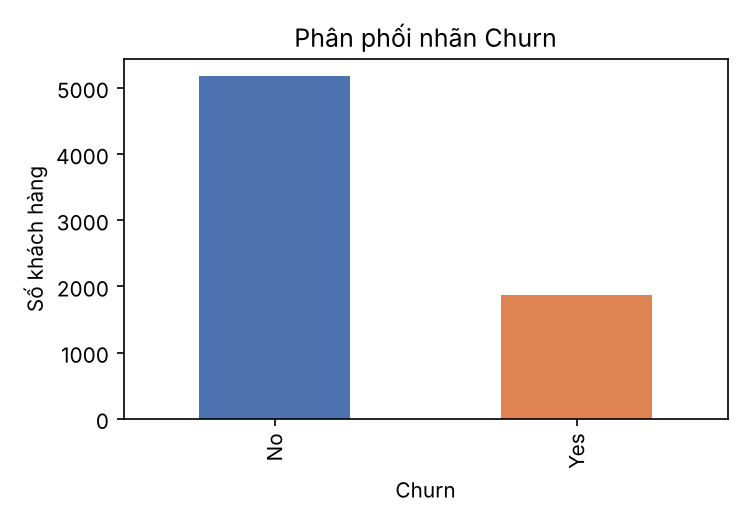
\includegraphics[width=0.6\textwidth]{../results/figures/eda_phan_phoi_nhan.png}
    \caption{Phân phối nhãn Churn}
    \label{fig:eda-nhan}
    \Nguon{Dữ liệu Telco Customer Churn; nhóm tự vẽ}
\end{figure}

\begin{figure}[H]
    \centering
    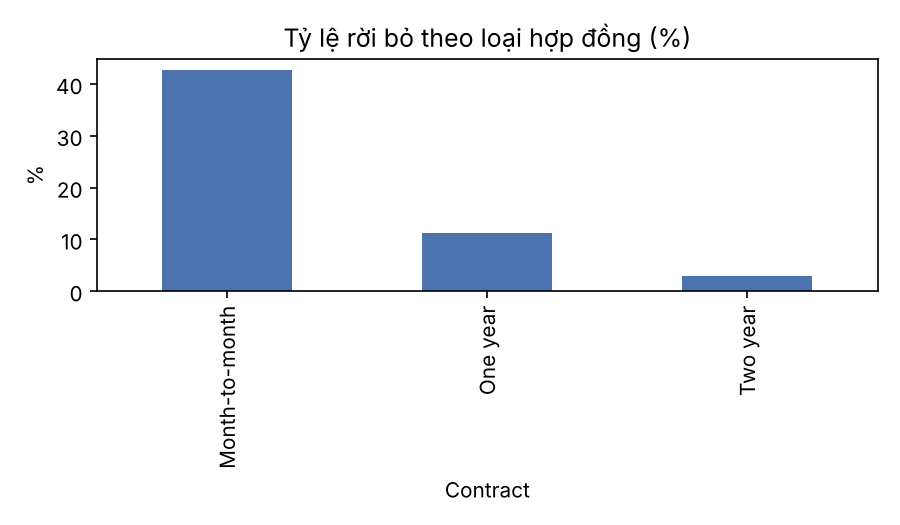
\includegraphics[width=0.7\textwidth]{../results/figures/eda_churn_theo_hop_dong.png}
    \caption{Tỷ lệ rời bỏ theo loại hợp đồng}
    \label{fig:eda-hopdong}
    \Nguon{Dữ liệu Telco Customer Churn; nhóm tự vẽ}
\end{figure}

\begin{figure}[H]
    \centering
    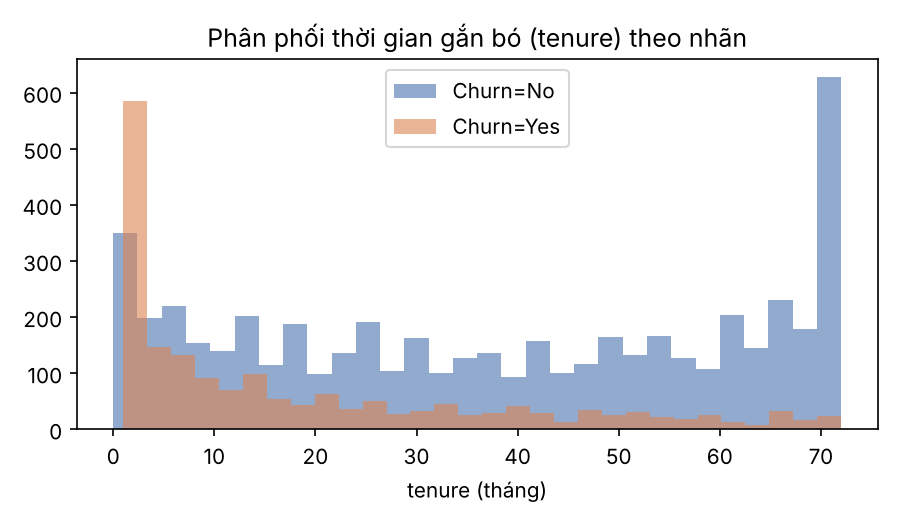
\includegraphics[width=0.7\textwidth]{../results/figures/eda_tenure.png}
    \caption{Phân phối thời gian gắn bó theo nhãn}
    \label{fig:eda-tenure}
    \Nguon{Dữ liệu Telco Customer Churn; nhóm tự vẽ}
\end{figure}

Từ biểu đồ, nhóm đưa ra hai giả thuyết được kiểm chứng ở chương 4: khách hàng theo hợp đồng tháng có nguy cơ rời bỏ cao hơn,
và nguy cơ giảm khi thời gian gắn bó tăng. Kết quả thống kê trên bộ dữ liệu gồm 7.043 khách hàng và 21 cột (không có dòng trùng lặp):
\begin{itemize}
    \item Tỷ lệ rời bỏ chung là 26,5\% (1.869 khách hàng). Nhãn có mất cân bằng nhưng không quá nghiêm trọng.
    \item Theo loại hợp đồng: hợp đồng theo tháng có tỷ lệ rời bỏ 42,7\%, hợp đồng một năm 11,3\% và hợp đồng hai năm 2,8\%.
    \item Theo loại internet: nhóm cáp quang (Fiber optic) có tỷ lệ rời bỏ 41,9\%, DSL 19,0\%, và nhóm không dùng internet 7,4\%.
    \item Theo thời gian gắn bó: nhóm 0--12 tháng có tỷ lệ rời bỏ 47,4\%, nhóm trên 48 tháng chỉ 9,5\%.
\end{itemize}
Hai giả thuyết ở trên được xác nhận bởi số liệu: hợp đồng theo tháng và thời gian gắn bó ngắn là hai yếu tố liên quan mạnh nhất đến việc rời bỏ.
